% !TeX root = ../main.tex
% %%%%%%%%%%%%%%%%%%%%%%%%%%%%%%%%%%%%%%%%%%%%%%%%%%%%%%%%%%%%%%%%%%%%%%%%%%%%%%
% Appendixes
\chapter*{Appendix A}
\label{app:appendix-A}

\begin{comment}

\textbf{{\Huge Displayed Error messages}}

\begin{figure}
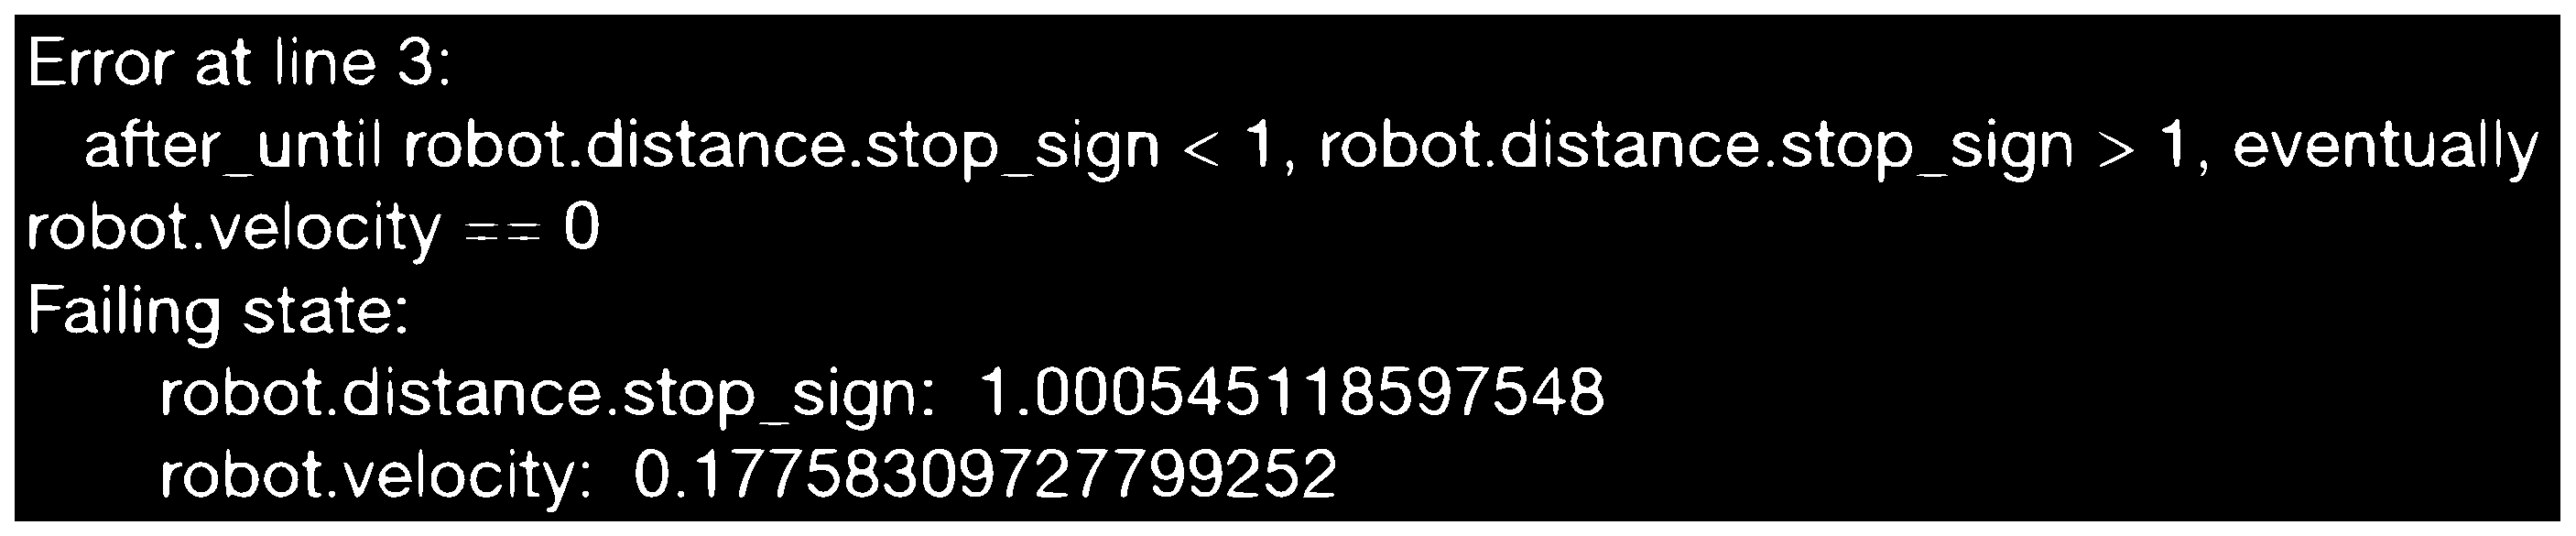
\includegraphics[width=\textwidth]{images/error.eps}
\caption{Example of the displayed error when the robot does not stop at the stop sign.}
\end{figure}

\begin{figure}[h]
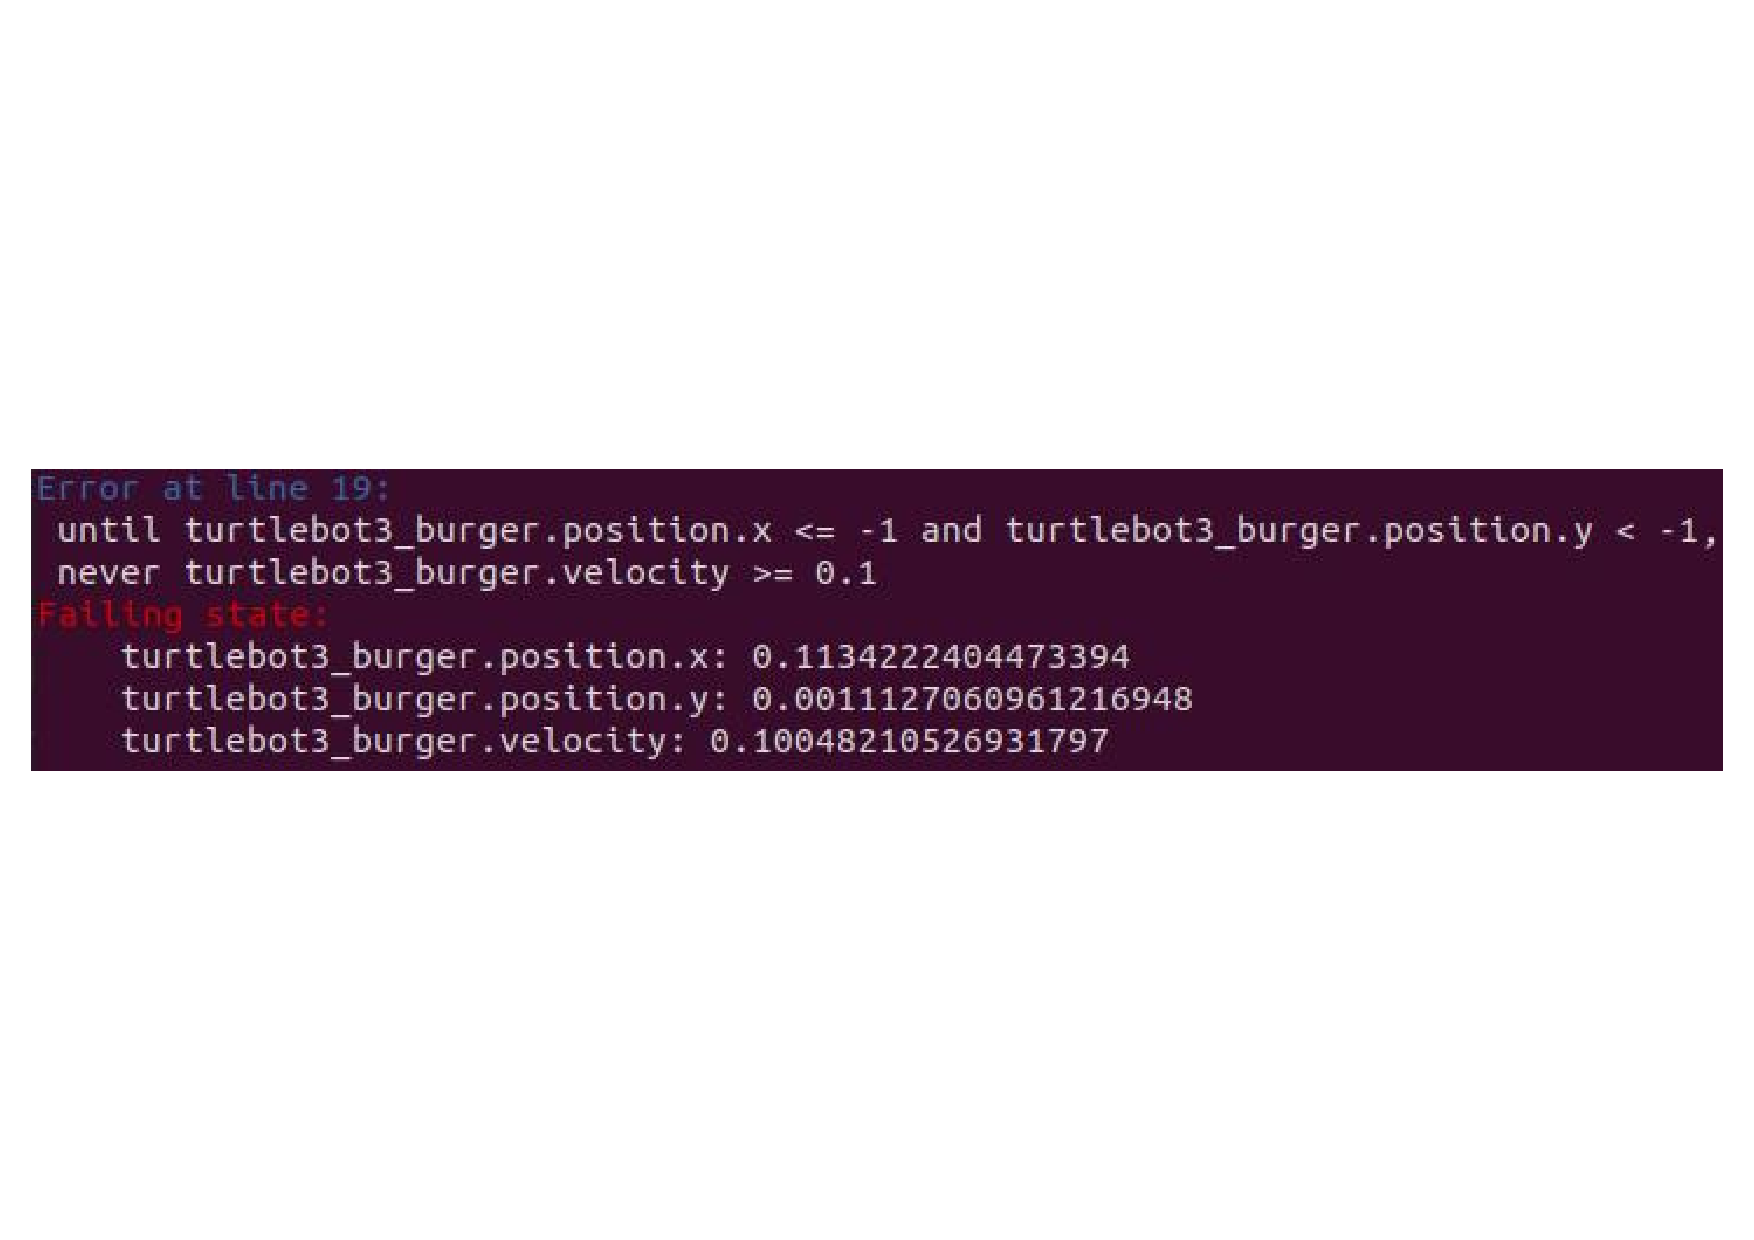
\includegraphics[width=\textwidth]{images/error_message.pdf}
\caption{Example of an error message.}
\end{figure}

\begin{figure}
\begin{center}
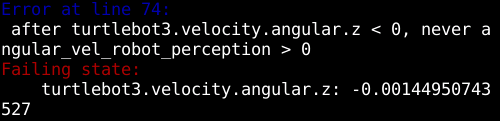
\includegraphics[width=8cm,height=2cm,keepaspectratio,]{images/erreval1.png}
\caption{Calculation Error Inverts Turning Direction bug error message.}
\end{center}
\end{figure}

\begin{figure}
\begin{center}
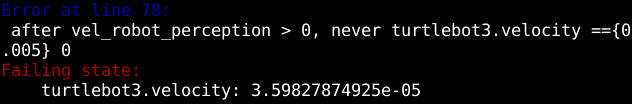
\includegraphics[width=10cm,height=3cm,keepaspectratio,]{images/erreval2.png}
\caption{Robot Getting Stuck When Auto-docking bug error message.}
\end{center}
\end{figure}

\begin{figure}
\begin{center}
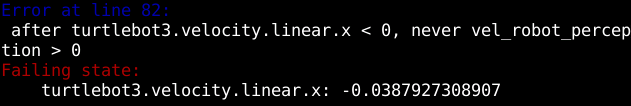
\includegraphics[width=10cm,height=3cm,keepaspectratio,]{images/erreval3.png}
\caption{Unexpected Movement Due to Wrong Calculation bug error message.}
\end{center}
\end{figure}


\chapter*{Appendix B}
\label{app:appendix-B}

\textbf{{\Huge Evaluation Flow Diagrams}}

\begin{figure}
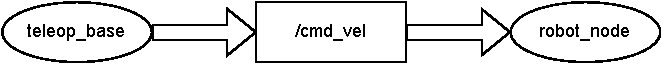
\includegraphics[width=\textwidth]{images/normal_flow.pdf}
\caption{The normal runtime flow of the system.}
\end{figure}
       
\begin{figure}
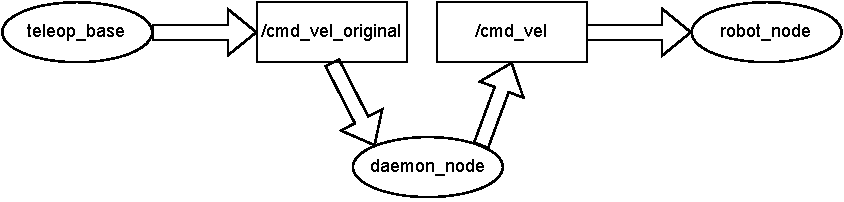
\includegraphics[width=\textwidth]{images/demon_flow.pdf}
\caption{The flow of the system when the adding the demon node.}
\end{figure}

\end{comment}
